\chapter{Air, a Mixture of Gases}\label{ch:g4:air-a-mixture-of-gases}

On a windy day a kite tugs at its string, and on the lake a sail fills
and pushes a boat along. Something is pushing them, yet there is nothing
to see. That something is \omterm{def:g4:air-a-mixture-of-gases:air}{air}. We cannot see it, but it is all around
us, it fills every empty bottle and every room, and we take it in with
every breath. What is \omterm{def:g4:air-a-mixture-of-gases:air}{air} made of?

\begin{recall}
To \omterm{def:g2:mixing-and-dissolving:mix}{mix} is to put different things together; what we get is a \omterm{def:g2:mixing-and-dissolving:mix}{mix} of
those things, and nothing is lost when we \omterm{def:g2:mixing-and-dissolving:mix}{mix} them
(\cref{ch:g2:mixing-and-dissolving}).
\end{recall}

\begin{omfigure}
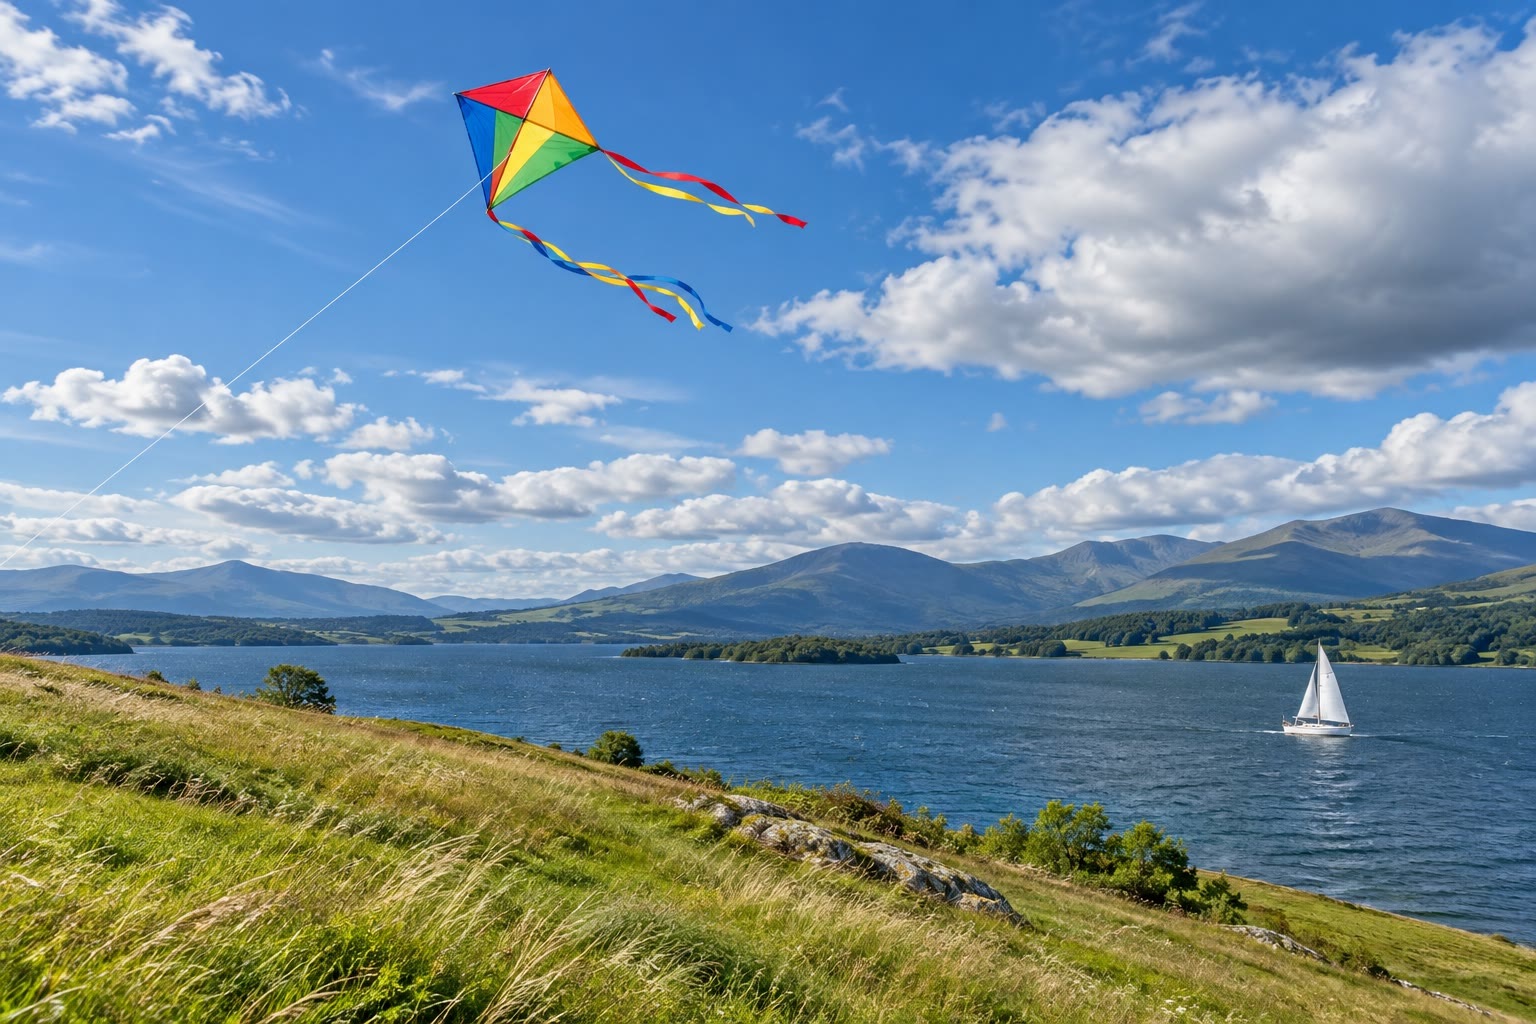
\includegraphics[width=0.6\linewidth]{images/book1/ai/g4-kite-day.jpg}

{\small A kite and a sail: \omterm{def:g4:air-a-mixture-of-gases:air}{air} cannot be seen, but it pushes.}
\end{omfigure}

\section{Air is all around us}

\begin{example}[An upturned glass]\label{ex:g4:air-a-mixture-of-gases:glass}
A dry paper tissue is pushed to the bottom of an empty glass. The glass
is turned upside down and pushed straight down into a bowl of water.
When it is lifted out again, the tissue is still dry. The glass was not
empty: it was full of \omterm{def:g4:air-a-mixture-of-gases:air}{air}, and the \omterm{def:g4:air-a-mixture-of-gases:air}{air} kept the water out.
\end{example}

\begin{omfigure}
\begin{tikzpicture}[font=\small, scale=1.3]
  \pic[transform shape] at (0,0) {trough};
  % the upturned glass, rim at y = 0.35, base at y = 2.35
  \fill[white] (-0.8,0.5) rectangle (0.8,0.95);
  \pic[transform shape, rotate=180] at (0,2.35) {beaker={0}{white}};
  % the tissue at the top, inside
  \fill[white, draw=black!45, rounded corners=1.5pt] (-0.4,2.33) -- (-0.3,2.05)
    -- (-0.1,2.12) -- (0.05,1.98) -- (0.25,2.1) -- (0.42,2.02) -- (0.45,2.33) -- cycle;
  \draw[<-, omProp, thick] (0.45,2.12) -- (2.4,2.5) node[right, text=black]
    {a dry tissue};
  \draw[<-, omProp, thick] (0.3,1.2) -- (2.4,1.4) node[right, text=black]
    {air: it keeps the water out};
  \draw[<-, omProp, thick] (1.4,0.7) -- (2.4,0.55) node[right, text=black]
    {water};
\end{tikzpicture}

{\small The glass is pushed upside down into the water. The \omterm{def:g4:air-a-mixture-of-gases:air}{air} trapped
inside keeps the water out, and the tissue stays dry.}
\end{omfigure}


\begin{remark}[Air is a gas]\label{rem:g4:air-a-mixture-of-gases:gas}
\omterm{def:g4:air-a-mixture-of-gases:air}{Air} is a gas: it has no shape of its own and spreads out to fill any
container. It is matter all the same, and a balloon full of \omterm{def:g4:air-a-mixture-of-gases:air}{air} weighs a
little more than the same balloon empty. What gases are, and why they
behave like this, is told in the physics book.
\end{remark}

\section{Air is a mixture}

\begin{definition}[Air]\label{def:g4:air-a-mixture-of-gases:air}
\emph{Air}\index{air} is the mixture of gases that surrounds the Earth.
It is not one single gas: several gases are mixed in it, and they can
be separated from one another.
\end{definition}

\begin{proposition}[What air is made of]\label{prop:g4:air-a-mixture-of-gases:composition}
% ledger: air:N2, air:O2, air:Ar, air:trace, air:CO2, air:H2O
Leaving out its water vapour, \omterm{def:g4:air-a-mixture-of-gases:air}{air} is made of:
\begin{itemize}
  \item \textbf{nitrogen}, about four fifths of the \omterm{def:g4:air-a-mixture-of-gases:air}{air};
  \item \textbf{oxygen}, about one fifth of the \omterm{def:g4:air-a-mixture-of-gases:air}{air};
  \item a little \textbf{argon}, about 1 part in 100;
  \item a very little \textbf{carbon dioxide}, about 4 parts in 10\,000,
        and tiny amounts of other gases.
\end{itemize}
\omterm{def:g4:air-a-mixture-of-gases:air}{Air} also holds \textbf{water vapour}, invisible: very little on a dry
cold day, up to about 4 parts in 100 on a hot damp day.
\end{proposition}

\begin{example}[One hundred bottles of air]\label{ex:g4:air-a-mixture-of-gases:hundred}
% ledger: air:N2, air:O2, air:Ar
Imagine 100 bottles of dry \omterm{def:g4:air-a-mixture-of-gases:air}{air}, and the gases of the \omterm{def:g4:air-a-mixture-of-gases:air}{air} sorted into
separate bottles. About 78 bottles would hold nitrogen, 21 bottles
oxygen, and the last bottle argon, with a few drops' worth of carbon
dioxide and other gases.
\end{example}

\begin{omfigure}
\begin{tikzpicture}[font=\small, x=0.42cm, y=0.42cm]
  \foreach \k in {0,...,99} {
    \pgfmathtruncatemacro\col{mod(\k,10)}
    \pgfmathtruncatemacro\row{9-int(\k/10)}
    \ifnum\k<78 \def\c{omDef!45}\else\ifnum\k<99 \def\c{red!45}\else\def\c{cyan!60}\fi\fi
    \fill[\c, draw=white, line width=0.8pt] (\col,\row) rectangle ++(1,1);
  }
  \fill[omDef!45] (12,8) rectangle ++(1,1);
  \node[anchor=west] at (13.3,8.5) {nitrogen: 78 squares};
  \fill[red!45] (12,6) rectangle ++(1,1);
  \node[anchor=west] at (13.3,6.5) {oxygen: 21 squares};
  \fill[cyan!60] (12,4) rectangle ++(1,1);
  \node[anchor=west, align=left] at (13.3,4.5) {argon, carbon dioxide\\ and the rest: 1 square};
\end{tikzpicture}

{\small One hundred squares of dry \omterm{def:g4:air-a-mixture-of-gases:air}{air}. The square at the bottom right
holds the argon, and the carbon dioxide too small to draw on its own.}
\end{omfigure}

\begin{remark}[Names of gases]\label{rem:g4:air-a-mixture-of-gases:names}
Nitrogen, oxygen, argon and carbon dioxide are the names of gases. They
are all colourless and have no smell. A later chapter shows what each of
them is made of, down to the tiny pieces that make up all matter.
\end{remark}

\section{What we breathe in and out}

\begin{proposition}[Breathed-out air]\label{prop:g4:air-a-mixture-of-gases:breath}
% ledger: breath:O2, breath:CO2, breath:N2, air:O2, air:CO2
The \omterm{def:g4:air-a-mixture-of-gases:air}{air} we breathe out is not the \omterm{def:g4:air-a-mixture-of-gases:air}{air} we breathed in. Our body takes
some of the oxygen and gives out carbon dioxide and water vapour:
\begin{itemize}
  \item about 21 parts in 100 of the \omterm{def:g4:air-a-mixture-of-gases:air}{air} breathed in are oxygen, but only
        about 16 parts in 100 of the \omterm{def:g4:air-a-mixture-of-gases:air}{air} breathed out;
  \item carbon dioxide goes from about 4 parts in 10\,000 to about 4
        parts in 100: about a hundred times more;
  \item the nitrogen is breathed out just as it was breathed in.
\end{itemize}
\end{proposition}

\begin{omfigure}
\begin{tikzpicture}
\begin{axis}[ybar, width=0.8\linewidth, height=5.2cm, bar width=12pt,
    ymin=0, ymax=90, ylabel={parts in 100},
    symbolic x coords={nitrogen, oxygen, carbon dioxide}, xtick=data,
    tick label style={font=\small}, label style={font=\small},
    xticklabel style={text height=1.6ex, text depth=0.4ex},
    legend style={font=\small, at={(0.98,0.95)}, anchor=north east},
    nodes near coords, nodes near coords style={font=\footnotesize},
    enlarge x limits=0.25, axis lines*=left, ymajorgrids,
    grid style={gray!20}]
% ledger: air:N2, air:O2, air:CO2, breath:N2, breath:O2, breath:CO2 (rounded)
\addplot[fill=omDef!45, draw=omDef] coordinates
  {(nitrogen,78) (oxygen,21) (carbon dioxide,0)};
\addplot[fill=omProp!55, draw=omProp] coordinates
  {(nitrogen,78) (oxygen,16) (carbon dioxide,4)};
\legend{breathed in, breathed out}
\end{axis}
\end{tikzpicture}

{\small Breathed in and breathed out, in parts in 100 (water vapour left
out, numbers rounded). The carbon dioxide of the \omterm{def:g4:air-a-mixture-of-gases:air}{air} breathed in, 4 parts
in 10\,000, is too small to show as a bar.}
\end{omfigure}

\begin{example}[A crowded room]\label{ex:g4:air-a-mixture-of-gases:room}
In a small classroom with the windows shut, thirty people breathe out
carbon dioxide all morning. Little by little the \omterm{def:g4:air-a-mixture-of-gases:air}{air} of the room holds
less oxygen and more carbon dioxide, and people feel tired. Opening the
windows brings fresh \omterm{def:g4:air-a-mixture-of-gases:air}{air} back in.
\end{example}

\begin{omfigure}
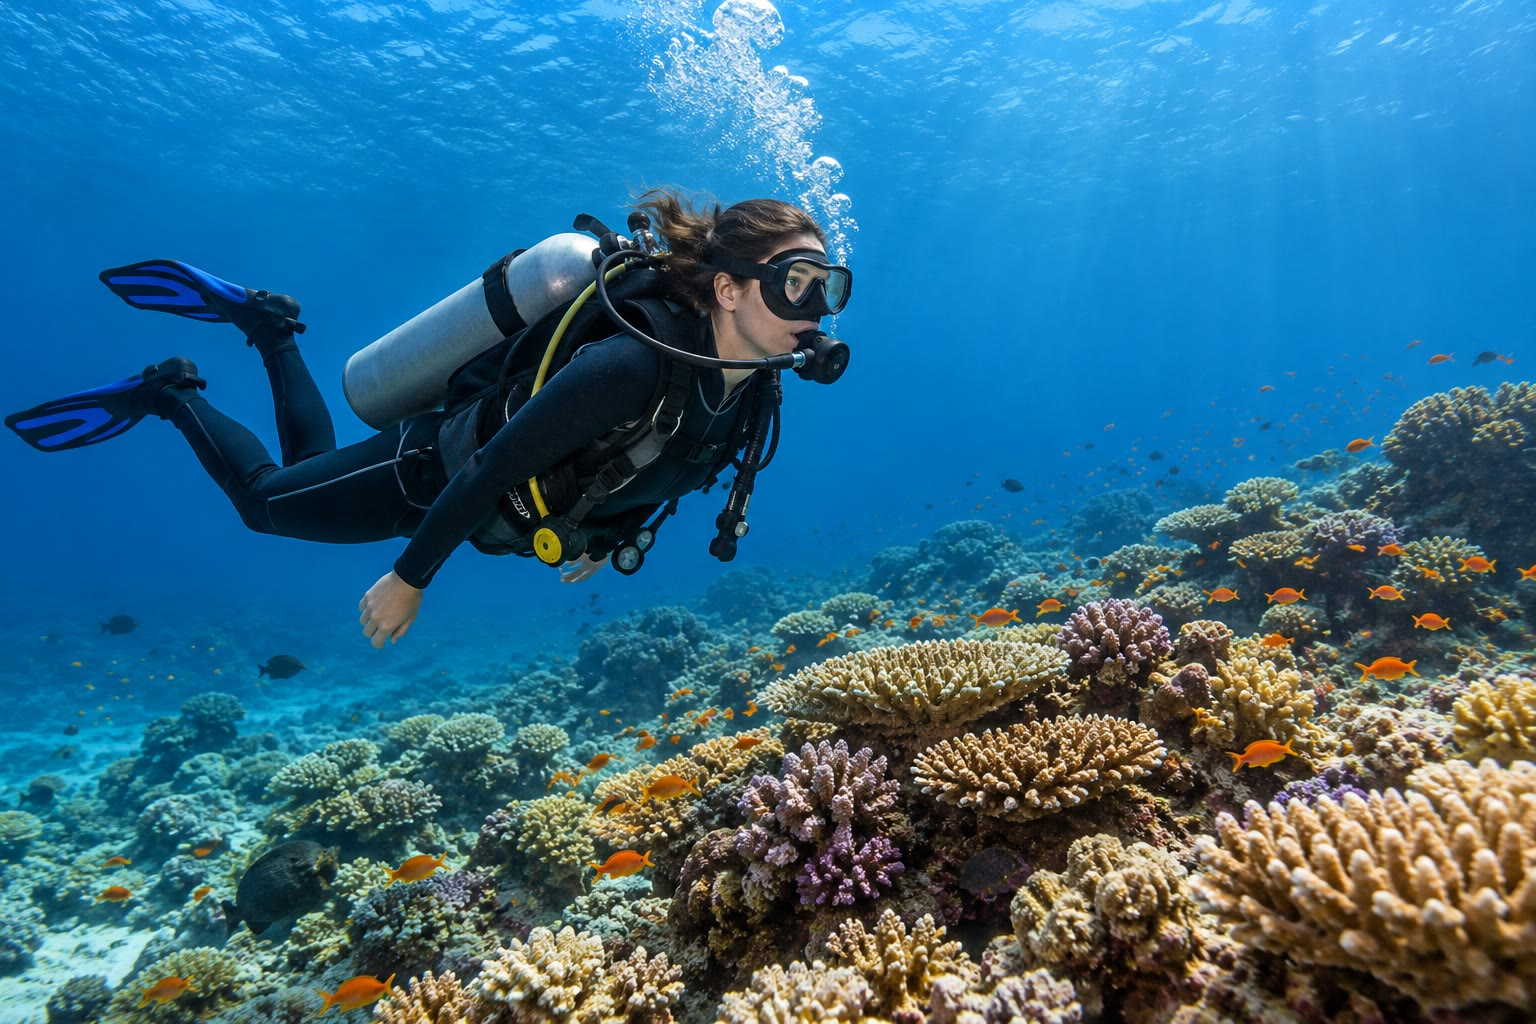
\includegraphics[width=0.55\linewidth]{images/book1/ai/g4-scuba-diver.jpg}

{\small A diver breathes \omterm{def:g4:air-a-mixture-of-gases:air}{air} from the tank on the back; the bubbles are
the \omterm{def:g4:air-a-mixture-of-gases:air}{air} breathed out.}
\end{omfigure}

\begin{remark}[Why divers breathe air]\label{rem:g4:air-a-mixture-of-gases:diver}
A diver's tank is filled with \omterm{def:g4:air-a-mixture-of-gases:air}{air} squeezed into a small space, not with
pure oxygen: breathing pure oxygen deep under water is dangerous. The
nitrogen of the \omterm{def:g4:air-a-mixture-of-gases:air}{air} is there to dilute the oxygen.
\end{remark}

\section{Oxygen for life and for fire}

\begin{proposition}[Oxygen is used up by living things and by flames]\label{prop:g4:air-a-mixture-of-gases:oxygen}
Of all the gases of the \omterm{def:g4:air-a-mixture-of-gases:air}{air}, oxygen is the one living things and flames
need. Animals and people take it in when they breathe; a flame takes it
from the \omterm{def:g4:air-a-mixture-of-gases:air}{air} around it. Green plants, in daylight, give oxygen back to
the \omterm{def:g4:air-a-mixture-of-gases:air}{air}.
\end{proposition}

\begin{inthelab}[A candle under a jar]
The teacher lights a candle on a tile and slowly lowers a large glass
jar over it. The flame shrinks, flickers and goes out after a few
seconds: around the flame, the \omterm{def:g4:air-a-mixture-of-gases:air}{air} holds too little oxygen to keep it
burning. Under a jar twice as large, the candle burns about twice as
long, because there is about twice as much \omterm{def:g4:air-a-mixture-of-gases:air}{air}, and so twice as much
oxygen, to use.
\end{inthelab}

\begin{omfigure}
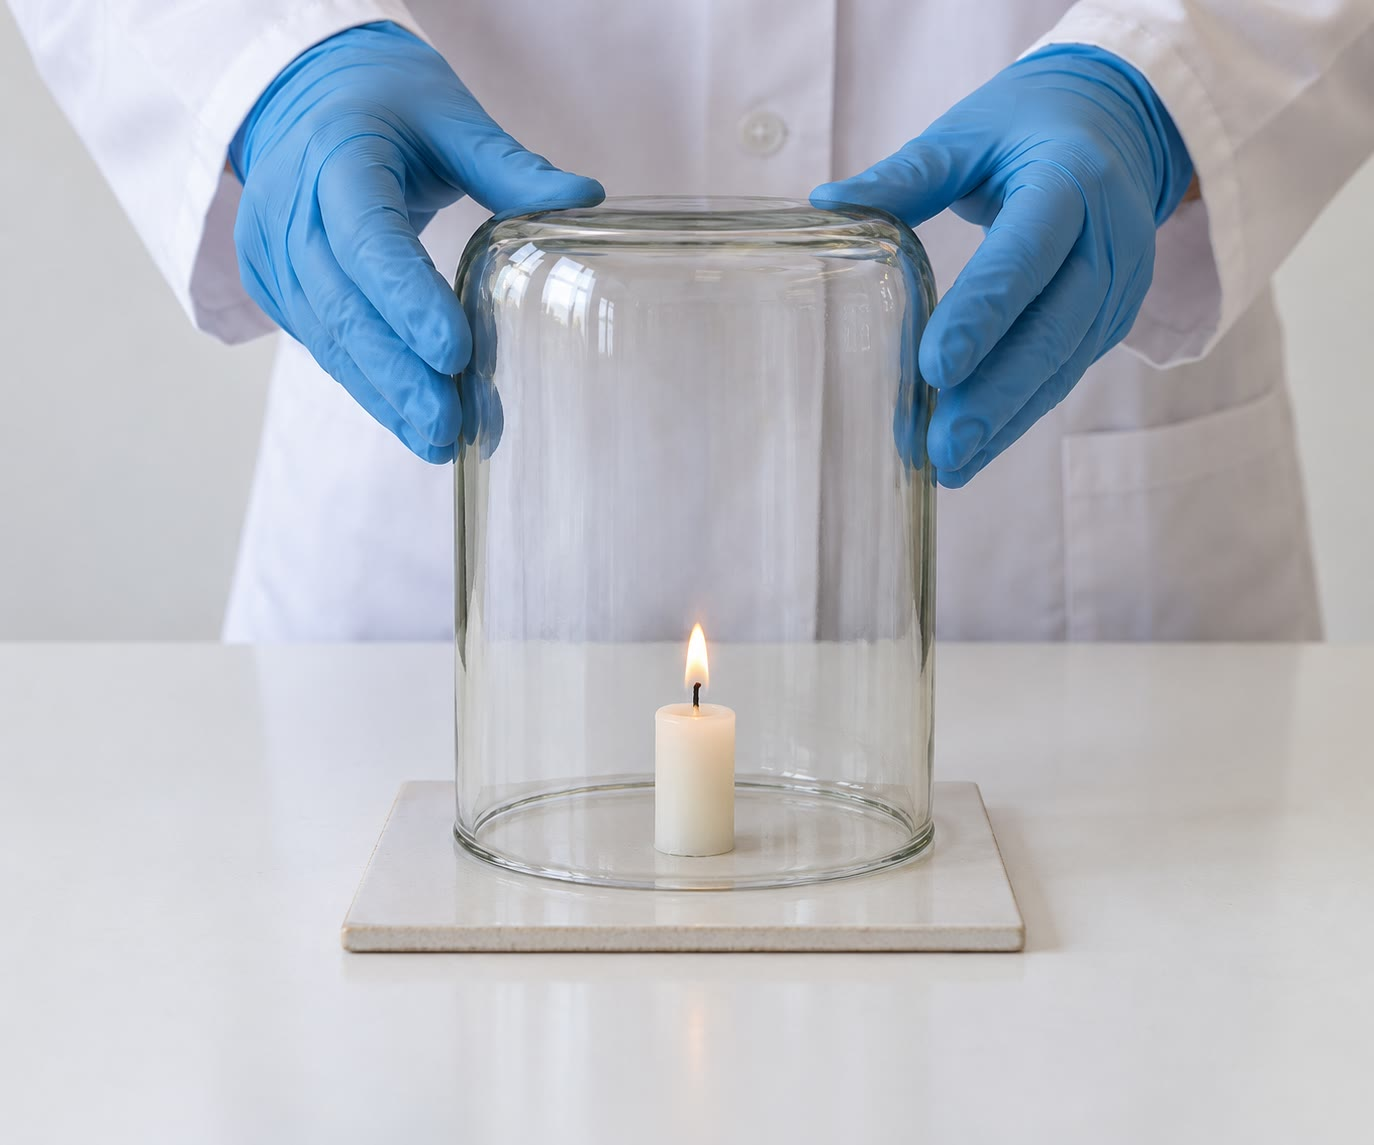
\includegraphics[width=0.5\linewidth]{images/book1/ai/g4-candle-jar-lab.jpg}

{\small A candle under a glass jar goes out when too little oxygen is
left around its flame.}
\end{omfigure}

\begin{remark}[Nitrogen does not burn]\label{rem:g4:air-a-mixture-of-gases:nitrogen}
Nitrogen is the largest part of the \omterm{def:g4:air-a-mixture-of-gases:air}{air}, yet it does not keep a flame
burning and it is not used by our body. If \omterm{def:g4:air-a-mixture-of-gases:air}{air} were all nitrogen, we
could not breathe and nothing could burn.
\end{remark}

\section{Exercises}

\begin{exercise}[$\star$]\label{exo:g4:air-a-mixture-of-gases:1}
Is \omterm{def:g4:air-a-mixture-of-gases:air}{air} one single gas or a mixture? Name the two main gases of the \omterm{def:g4:air-a-mixture-of-gases:air}{air}.
\end{exercise}

\begin{exercise}[$\star$]\label{exo:g4:air-a-mixture-of-gases:2}
About what fraction of the \omterm{def:g4:air-a-mixture-of-gases:air}{air} is nitrogen? About what fraction is
oxygen?
\end{exercise}

\begin{exercise}[$\star$]\label{exo:g4:air-a-mixture-of-gases:3}
In 100 litres of dry \omterm{def:g4:air-a-mixture-of-gases:air}{air}, about how many litres are nitrogen? About how
many litres are oxygen?
\end{exercise}

\begin{exercise}[$\star$]\label{exo:g4:air-a-mixture-of-gases:4}
An empty bottle is put upside down into a basin of water. Why does the
water not fill the bottle?
\end{exercise}

\begin{exercise}[$\star$]\label{exo:g4:air-a-mixture-of-gases:5}
Look at the bar chart. Which gas is there less of in the \omterm{def:g4:air-a-mixture-of-gases:air}{air} breathed
out? Which gas is there more of?
\end{exercise}

\begin{exercise}[$\star$]\label{exo:g4:air-a-mixture-of-gases:6}
Which gas of the \omterm{def:g4:air-a-mixture-of-gases:air}{air} does a flame need? Which gas of the \omterm{def:g4:air-a-mixture-of-gases:air}{air} do we need
when we breathe?
\end{exercise}

\begin{exercise}[$\star$]\label{exo:g4:air-a-mixture-of-gases:7}
Look at the figure with 100 squares. How many squares are nitrogen? How
many are not nitrogen?
\end{exercise}

\begin{exercise}[$\star$]\label{exo:g4:air-a-mixture-of-gases:8}
Why does a candle under a jar go out after a while?
\end{exercise}

\begin{exercise}[$\star$]\label{exo:g4:air-a-mixture-of-gases:9}
In 500 litres of \omterm{def:g4:air-a-mixture-of-gases:air}{air}, about how many litres are oxygen? (One fifth of
the \omterm{def:g4:air-a-mixture-of-gases:air}{air} is oxygen.)
\end{exercise}

\begin{exercise}[$\star\star$]\label{exo:g4:air-a-mixture-of-gases:10}
Why is it a good idea to open the windows of a classroom between
lessons?
\end{exercise}

\begin{exercise}[$\star\star$]\label{exo:g4:air-a-mixture-of-gases:11}
A candle burns for 10 seconds under a small jar. About how long would it
burn under a jar holding three times as much \omterm{def:g4:air-a-mixture-of-gases:air}{air}?
\end{exercise}
